\section{Metodología}

\subsection{Representación de las arquitecturas implementadas}

La Figura~\ref{fig:arquitecturas-av4} representa los tres diseños entrenados
desde cero. La entrada efectiva es una imagen RGB de $112\times112$ píxeles,
obtenida de los TFRecord de $224\times224$ mediante redimensionamiento bilineal
con antialias. Esto corrige la descripción anterior, que presentaba
$224\times224$ como resolución de entrenamiento.

\begin{figure*}[p]
\centering
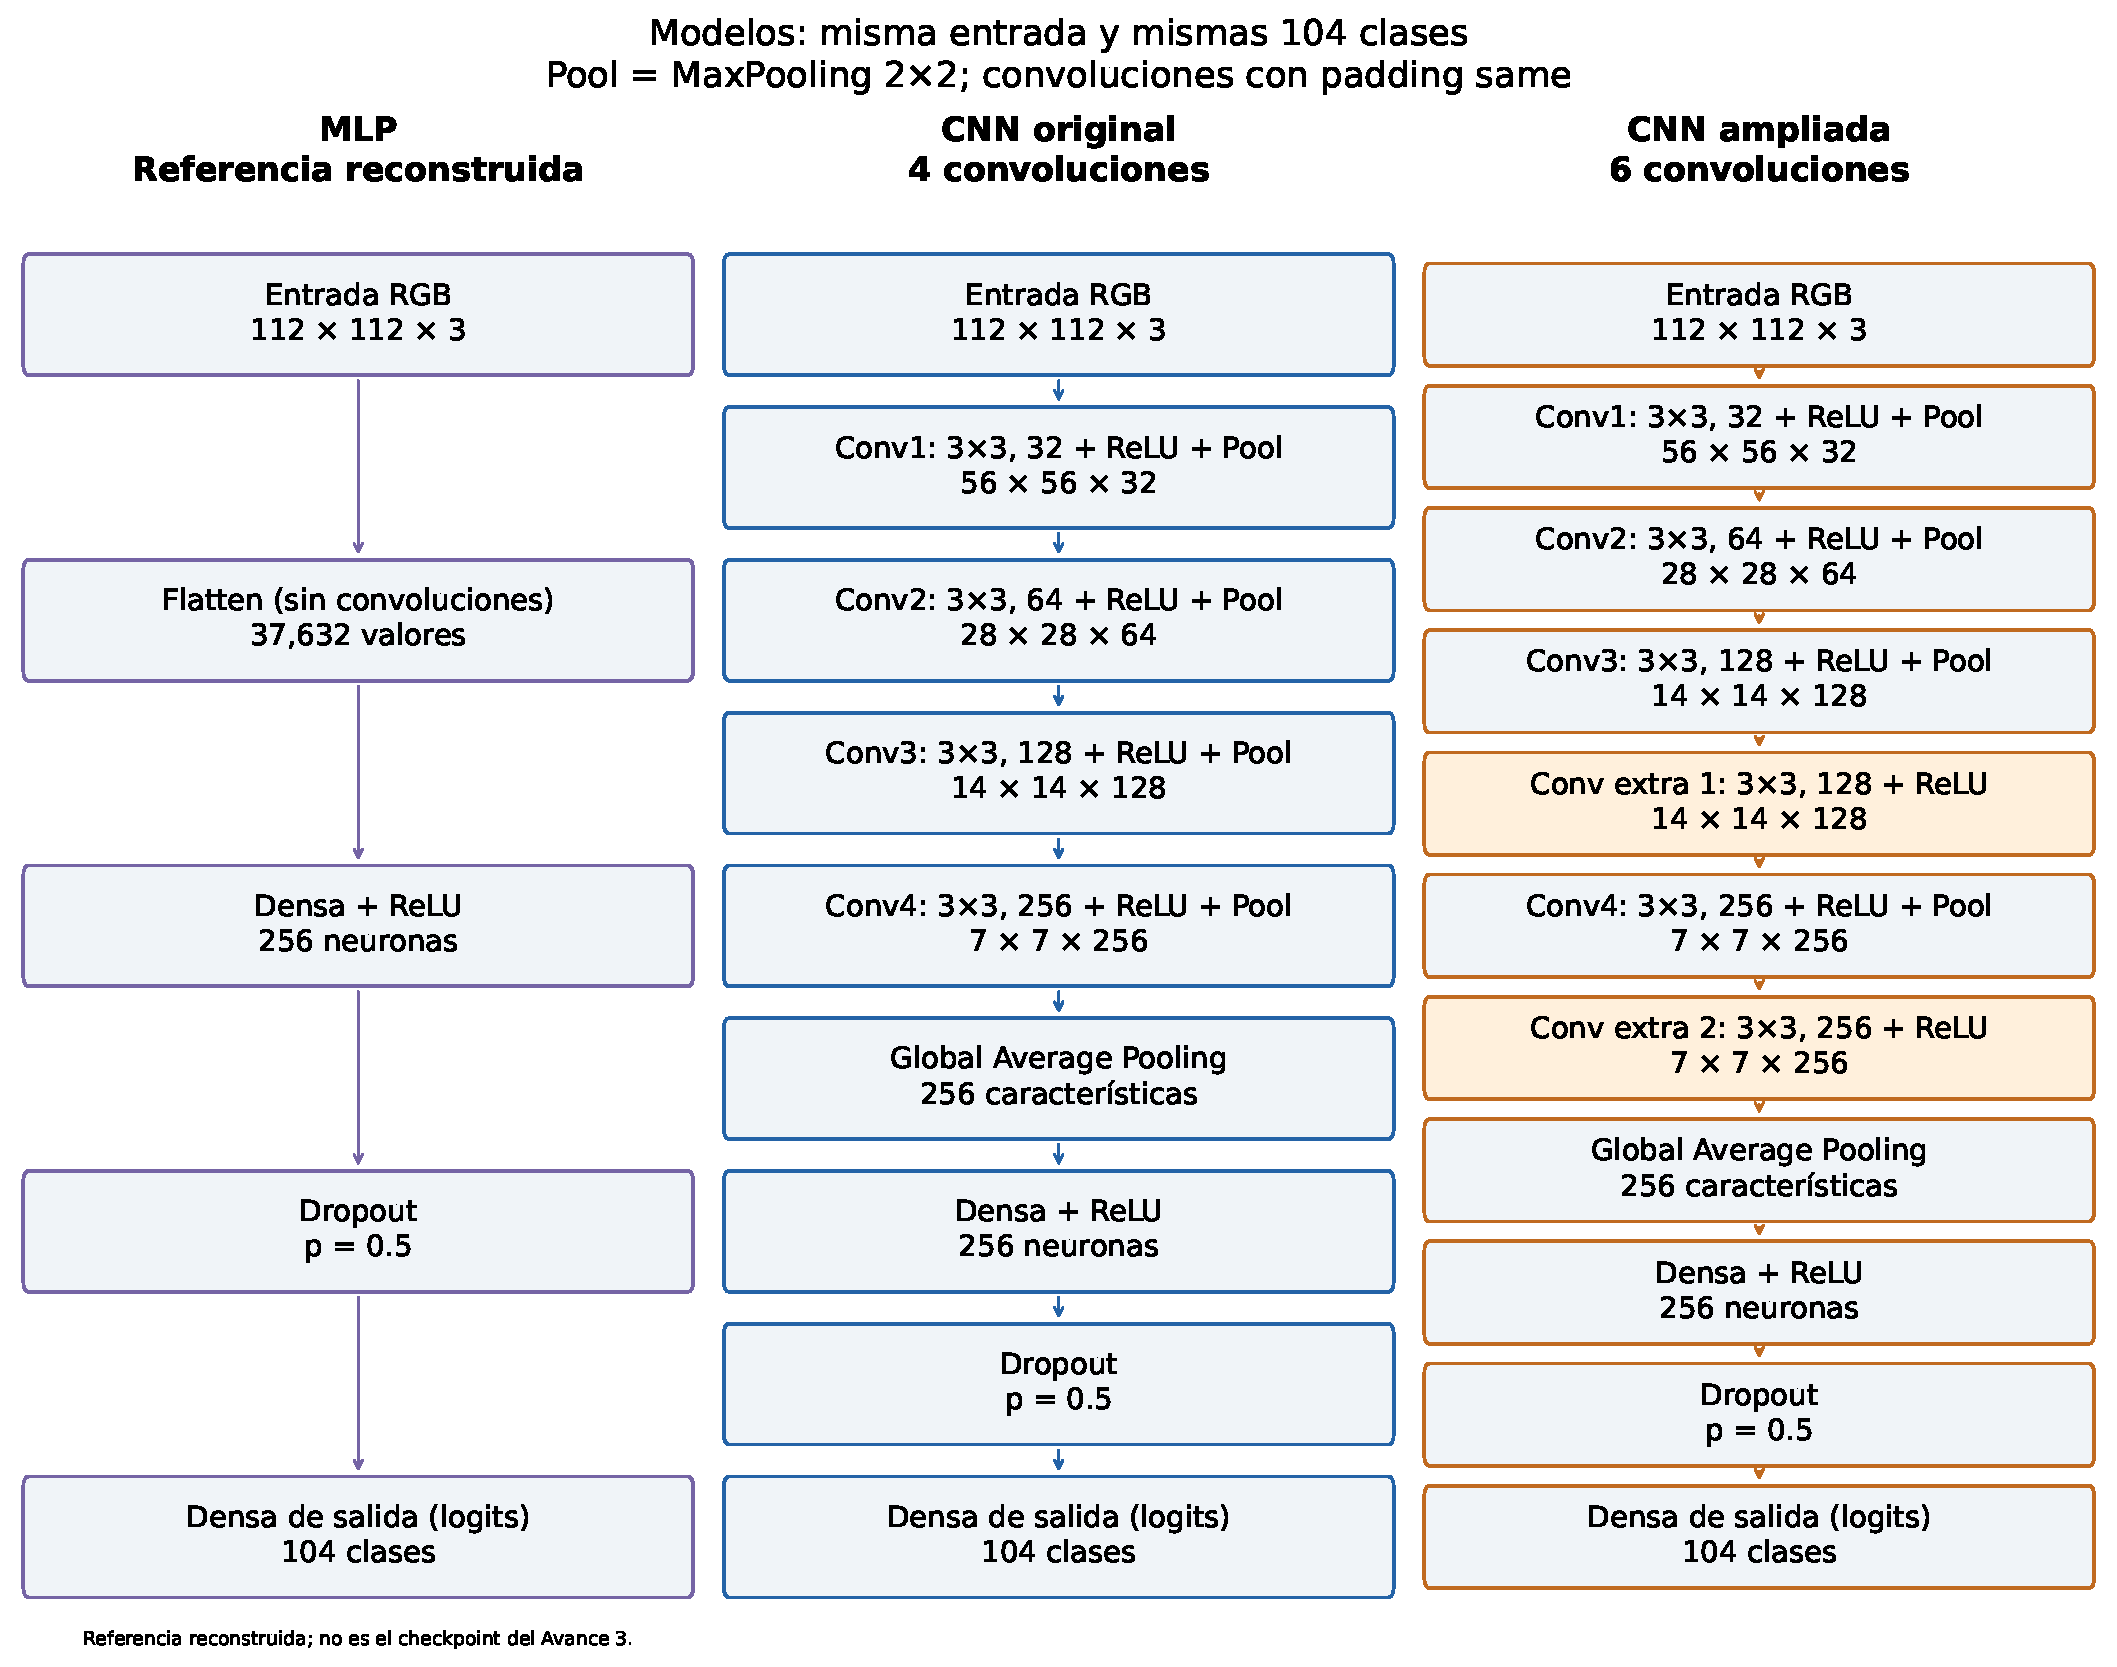
\includegraphics[width=\textwidth,height=0.85\textheight,keepaspectratio]{avance4_2026-10-21/figures/arquitecturas.pdf}
\caption{Representación de la red totalmente conectada de referencia, la CNN
original y la CNN con dos convoluciones adicionales. Las dimensiones corresponden
a las salidas de cada etapa; las capas adicionales se destacan en naranja.
La variante regularizada conserva la arquitectura de la CNN original.}
\label{fig:arquitecturas-av4}
\end{figure*}

La red \textbf{totalmente conectada de referencia} aplana los $112\times112\times3$
valores de entrada en un vector de 37,632 componentes. Aplica una capa densa de
256 unidades con ReLU, dropout de 0.5 y una salida de 104 logits. No contiene
convoluciones ni pooling. Es una comparación reconstruida, como se aclara en la
sección 1, y utiliza el mismo cargador, aumentos y ciclo de entrenamiento que la CNN.

La \textbf{CNN original} emplea cuatro convoluciones de $3\times3$, padding
\textit{same}, ReLU y 32, 64, 128 y 256 filtros. Cada convolución va seguida de
max pooling de $2\times2$. Las salidas de esos bloques son
$56\times56\times32$, $28\times28\times64$, $14\times14\times128$ y
$7\times7\times256$. Después aplica global average pooling (GAP), una capa densa
de 256 unidades con ReLU, dropout de 0.5 y 104 logits de salida.

La \textbf{CNN ampliada} agrega dos capas convolucionales ocultas: una de 128
filtros después del tercer pooling y otra de 256 después del cuarto. Ambas usan
kernel $3\times3$, padding \textit{same} y ReLU, sin pooling adicional. Por tanto,
esta versión tiene seis convoluciones. No se trata de dos capas densas nuevas.

La convolución comparte los pesos del filtro entre posiciones y analiza
vecindarios de píxeles. Así puede aprender bordes, texturas y partes de pétalos
antes de combinarlos. Una capa densa sobre píxeles aplanados asigna pesos
independientes a cada posición y no impone esta estructura local. Esta diferencia
motiva la comparación, pero la mejora debe comprobarse con las métricas.

\subsection{Preprocesamiento y aumento de datos}

Se decodifica cada JPEG como RGB, se convierten sus valores a float32, se
normalizan mediante $x_{\mathrm{norm}}=x/255$ y se redimensionan a $112\times112$.
Las etiquetas son enteros entre 0 y 103. Se mantiene la separación de archivos
original entre entrenamiento y validación, sin incorporar imágenes de validación
al entrenamiento.

Solo en entrenamiento se aplican volteo horizontal, rotación aleatoria de factor
0.05, zoom de 0.1 y contraste de 0.1. Los valores resultantes se recortan a $[0,1]$.
Los aumentos se calculan después de la caché y del mezclado, por lo que cambian
entre épocas. La validación usa imágenes deterministas sin aumentos.

\subsection{Pérdida y actualización de parámetros}

Los modelos producen 104 logits $z_k$. La entropía cruzada se calcula directamente
sobre ellos, sin añadir una segunda softmax a la pérdida:
\begin{equation}
L=-\log\left(\frac{\exp(z_c)}{\sum_{k=1}^{104}\exp(z_k)}\right),
\end{equation}
donde $c$ es la clase verdadera. Para visualizar la confianza se transforma la
salida mediante softmax; esta confianza no constituye una evaluación de calibración.

La referencia totalmente conectada y ambas CNN sin la intervención adicional
usan Adam con tasa inicial $10^{-3}$ y lotes de 64 imágenes. La variante
regularizada usa AdamW y un ajuste de tasa que se detalla en la sección 7.
Se entrena con PyTorch/DirectML en la GPU AMD Radeon RX 6700S, conservando el
cargador y los aumentos de TensorFlow. El mejor checkpoint se exporta a Keras
y se comprueba que mantiene los logits y las predicciones sobre un lote de control.

\subsection{Imágenes sintéticas: experimento independiente}

El proyecto también incluye destilación de datos mediante Distribution Matching
(DM). IPC 1 significa una imagen sintética por cada una de las 104 clases, es
decir, 104 imágenes; IPC 10 significa 1,040. El generador utiliza el extractor
convolucional de la arquitectura original con pesos aleatorios que se renuevan
durante la optimización de los píxeles. No utiliza como generador el checkpoint
entrenado de aproximadamente 63\% de exactitud. Estas figuras históricas se
conservan separadas; los experimentos principales de este avance entrenan con
las 12,753 imágenes reales y no se atribuyen sus métricas a los conjuntos sintéticos.

